% !TeX encoding = UTF-8

\documentclass{protokol}

\usepackage{tikz}
\usetikzlibrary{calc}
\usetikzlibrary{arrows}

%====== Units =====
\usepackage{siunitx}
\sisetup{inter-unit-product =\ensuremath{\cdot}}
\sisetup{group-digits = integer}
\sisetup{output-decimal-marker = {,}}
\sisetup{exponent-product = \ensuremath{\cdot}}
\sisetup{separate-uncertainty}
\sisetup{tight-spacing = false}
%\sisetup{scientific-notation = true}
%\sisetup{round-mode=places,round-precision=4}
%\sisetup{evaluate-expression}


%====== Grafy =====
\usepackage{pgfplots}
\pgfplotsset{width=0.8\linewidth, compat=1.17}
\def\plotcscale{0.8}
\usepackage{pgfplotstable}
\usepackage[figurename=Obr.]{caption} % figure caption rename
%====== Rovnice align block ======
\usepackage{amsmath}
\setlength{\jot}{10pt} % rozestup mezi řádky

\graphicspath{ {./img/} }

%====== Vyplňte údaje ======
\jmeno{Jakub Charvot}
\kod{240844}
\rocnik{2.}
\obor{MET}
\skupina{MET/4}
\spolupracoval{Radek Kučera}

\merenodne{13.\,10.\,2022}
\odevzdanodne{27.\,10.\,2022}
\nazev{Ověřování základních vlastností OZ}
\cislo{2} %měřené úlohy

\predmet{Analogové elektronické obvody}
\ustav{Ústav mikroelektroniky}
\skola{FEKT VUT v Brně}

\def\para{x+0}
\def\parb{\para-80}


\begin{document}
	%====== Vygenerování tabulky ======
	\maketitle
	%====== Úvodní texty protokolu ======
	
	\section{Teoretický úvod}
	
	\subsection{Vlastnosti OZ}
	
	\begin{table}[h!]
		\centering
		\def\arraystretch{1.4}
		\centering
		\begin{tabular}{|c|c|c|}	
			\hline
			Parametr & Ideální OZ & Reálný OZ (1458)\\ [0.1ex]
			\hline
			Stejnosměrné zesílení $ A_0 $ & $ \infty $ & $ \approx \num{200000}$\\ [0.1ex]
			\hline
			Vstupní odpor $ R_{in} $ & $\infty$ & $ \approx \SI{1}{\mega\ohm} $\\ [0.1ex]
			\hline
			Výstupní odpor $ R_{out} $ & 0 & $ \approx \SI{75}{\ohm} $\\ [0.1ex]
			\hline
			Slew Rate $ SR $ & $ \infty $ & $ \approx \SI{0.5}{\volt\per\micro\second} $\\ [0.1ex]
			\hline

		\end{tabular}
		\caption{Ideální a reálné parametry OZ.}
		\label{tab:porovnani}
	\end{table}

Důležitým paramaterem je $SR - Slew\ Rate $, mezní rychlost přeběhu. Maximální možná rychlost změny výstupního napětí. OZ neumí přenést ideální napěťový skok (obdélníkový signál) a vždy vytváří drobné nelineární zkreslení, u nízkých frekvencí a hodnot signálu to ale můžeme zanedbat.

Pro přenos sinusového ignálu pak platí $ 2\pi f U_2 < SR $, vycházíme z derivace v bodě průchodu signálu nulou.

\begin{figure}[h!]
	\centering
	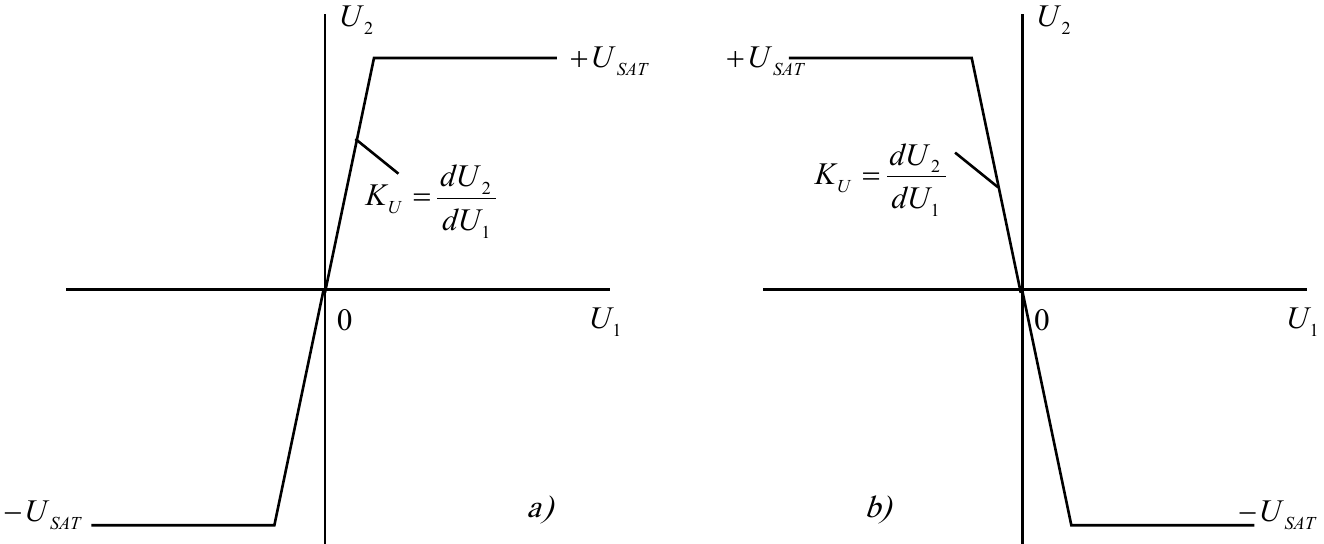
\includegraphics[width=0.8\textwidth]{prevodni.png}
	\centering
	\caption{Převodní charakteristiky OZ -- a) Neinvertující zapojení, b) Invertující zapojení.}
	\label{fig:prevodni}
\end{figure}


	\subsection{Zapojení OZ}
%	\subsubsection{Důležité parametry a vztahy}

		\begin{figure}[h!]
			\centering
			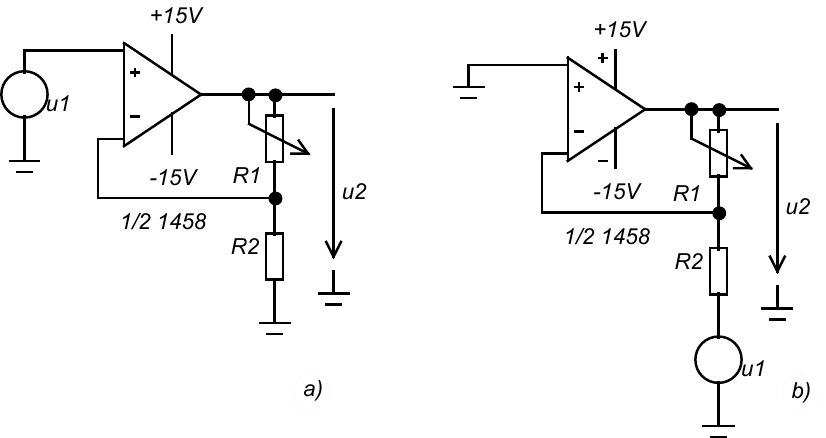
\includegraphics[width=0.7\textwidth]{schema.png}
			\centering
			\caption{Schéma zapojení. a) Neinvertující zesilovač, b) Invertující zesilovač.}
			\label{fig:schema}
		\end{figure}
	
	Samotný OZ má příliš vysoké zesílení a i při malé změně na vstupu už dosahuje saturace a tedy nefunguje správně. Pro stabilizaci jeho funkce využíváme záporné zpětné vazby -- část výstupního signálu přivádíme zpět na vstup a tím snižujeme rozdíl potenciálů na vstupních svorkách téměř na nulu.
	
	Napěťové zesílení dané aplikace vypočítáme následovně:\\\\
	$ K_U=1+\frac{R_1}{R_2}$\dots neinvertující zesilovač (Obr.~\ref{fig:schema} a))\\
	$ K_U=-\frac{R_1}{R_2}$\dots invertující zesilovač (Obr.~\ref{fig:schema} b))\\	
		
	
	\subsection{Kmitočtová charakteristika}
	
	\begin{figure}[h!]
		\centering
		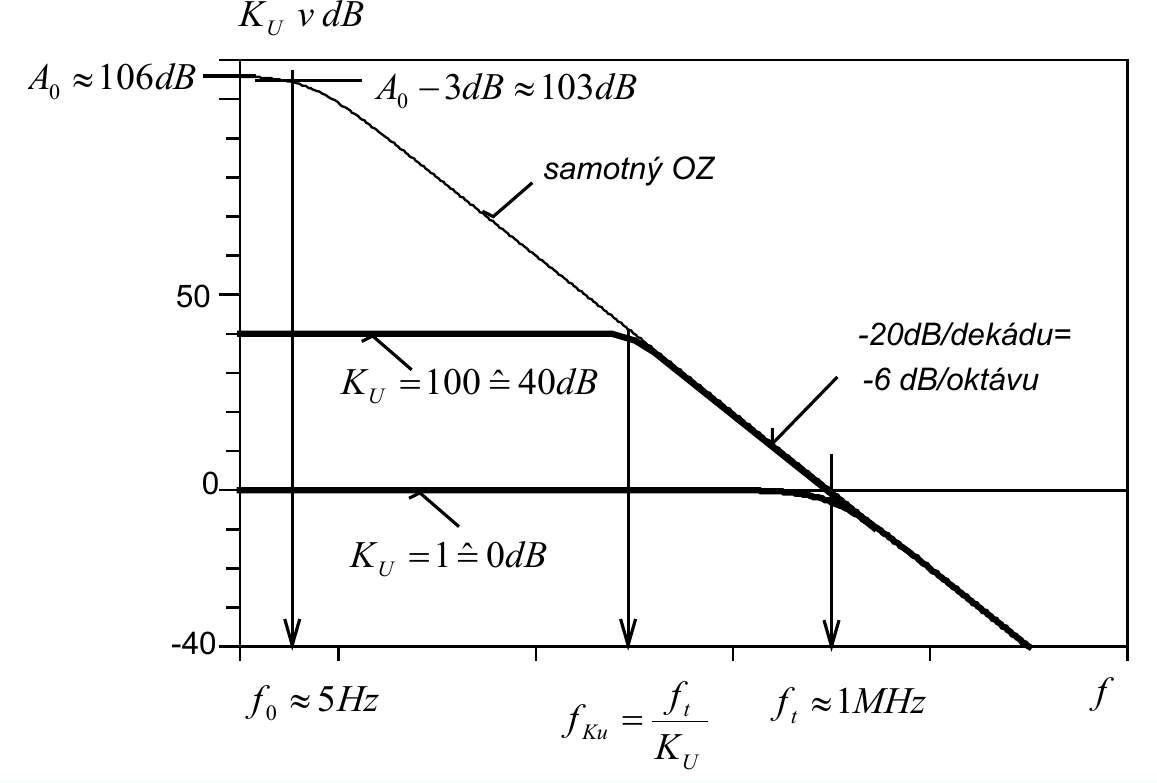
\includegraphics[width=0.7\textwidth]{kmitoctova.png}
		\centering
		\caption{Kmitočtová charakteristika 0Z 1458 a jeho neinvertujích zapojení.}
		\label{fig:kmitoctova_charakteristika}
	\end{figure}

	Samotný OZ má udávaný tranzitní kmitočet $ f_t=\SI{1}{\mega\hertz} $, tento údaj by ale platil jako horní mezní frekvence jen v případě zesílení 1. V případě aplikace s vyšším zesílením se horní mezní kmitočet snižuje dle vztahu:
	$$ f_{Ku} = \frac{f_t}{K_U}$$ 

	Grafické znázornění je na Obr.~\ref{fig:kmitoctova_charakteristika}.	
	
	
%	
	
	\newpage
\section{Výsledky počítačové simulace a laboratorního měření}
\subsection{Buffer}

	\begin{figure}[h!]
		\centering
		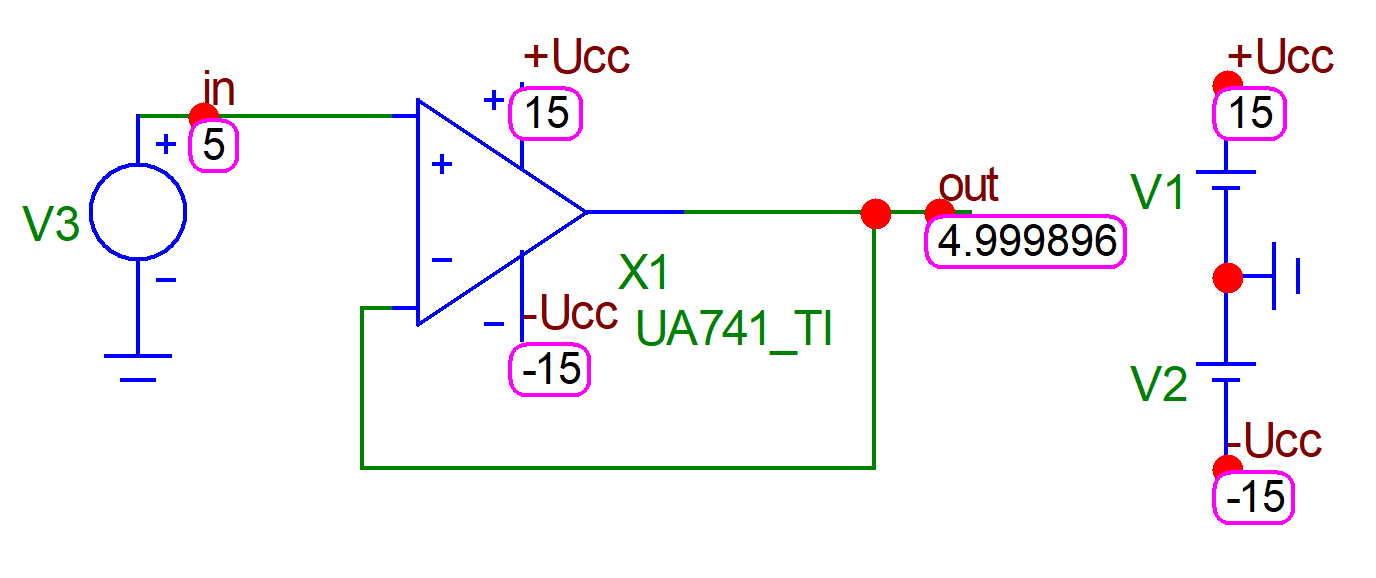
\includegraphics[width=0.8\textwidth]{numerika/Buffer/1_PracBod.png}
		\centering
		\caption{Buffer, simulace -- Pracovní bod obvodu.}
		\label{fig:mc_bt_prac_bod}
	\end{figure}

	\begin{figure}[h!]
		\centering
		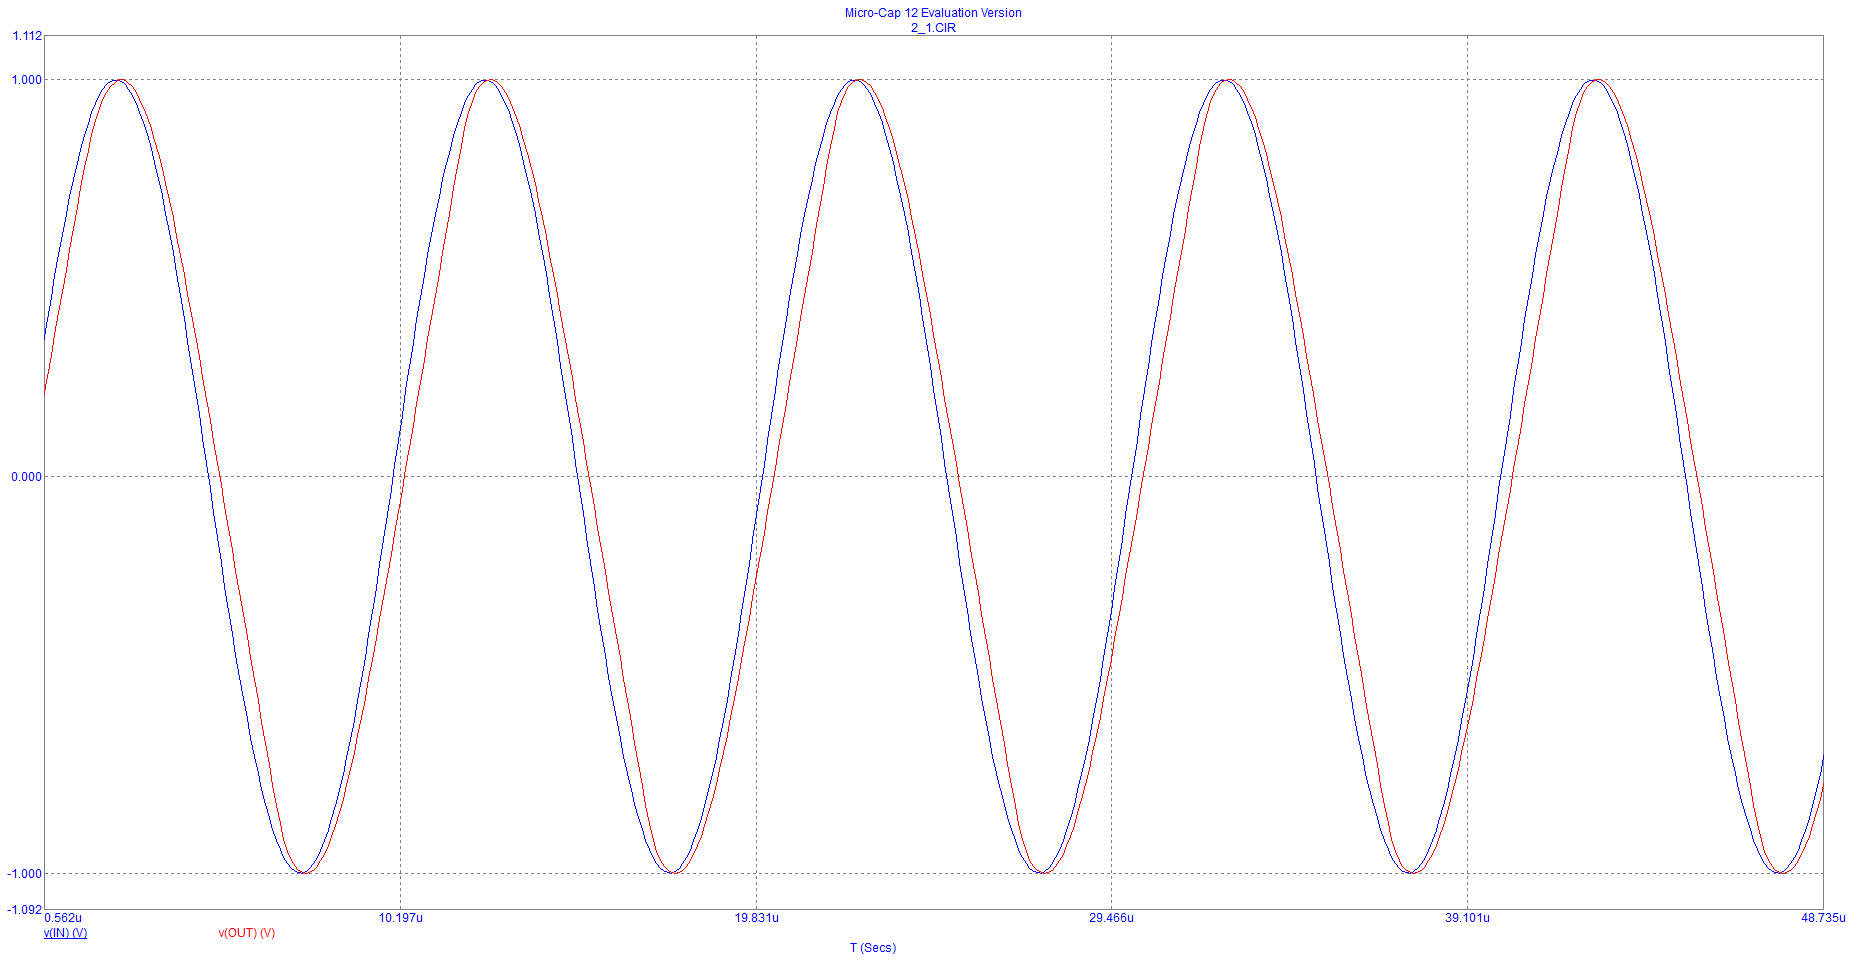
\includegraphics[width=0.7\textwidth]{numerika/Buffer/3_100k_sin_1V.png}
		\centering
		\caption{Buffer, simulace -- Přenos signálu o frekvenci $ \qty{100}{\kilo\hertz} $.}
		\label{fig:b-s-prenos1}
	\end{figure}
	
	\begin{figure}[h!]
		\centering
		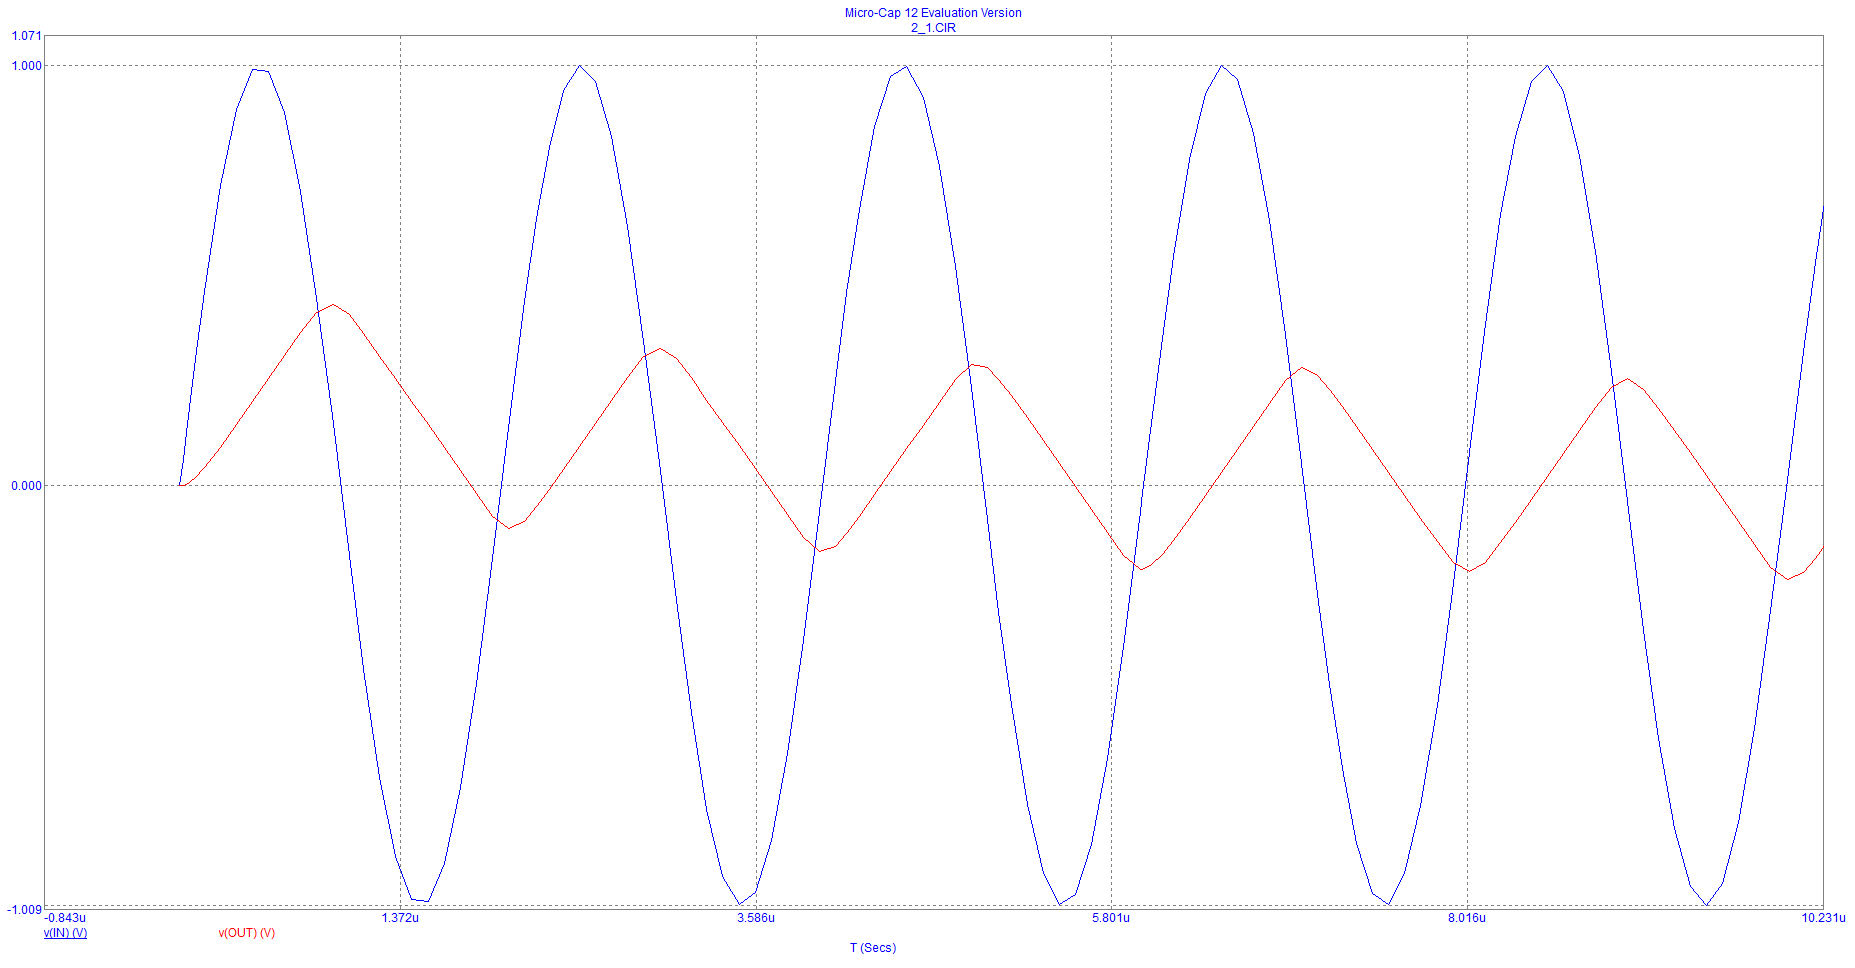
\includegraphics[width=0.7\textwidth]{numerika/Buffer/4_500k_sin_1V.png}
		\centering
		\caption{Buffer, simulace -- Přenos signálu o frekvenci $ \qty{500}{\kilo\hertz} $.}
		\label{fig:b-s-prenos2}
	\end{figure}

	\begin{figure}[h!]
		\centering
		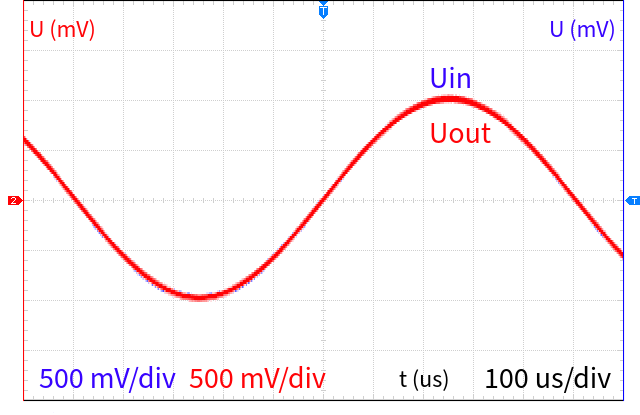
\includegraphics[width=\textwidth]{oscilo/output1.png}
		\centering
		\caption{Buffer, laboratoř -- Časová závislost vstupního a výstupního napětí.}
		\label{fig:b-l-prenos}
	\end{figure}



	\begin{figure}[h!]
		\centering
		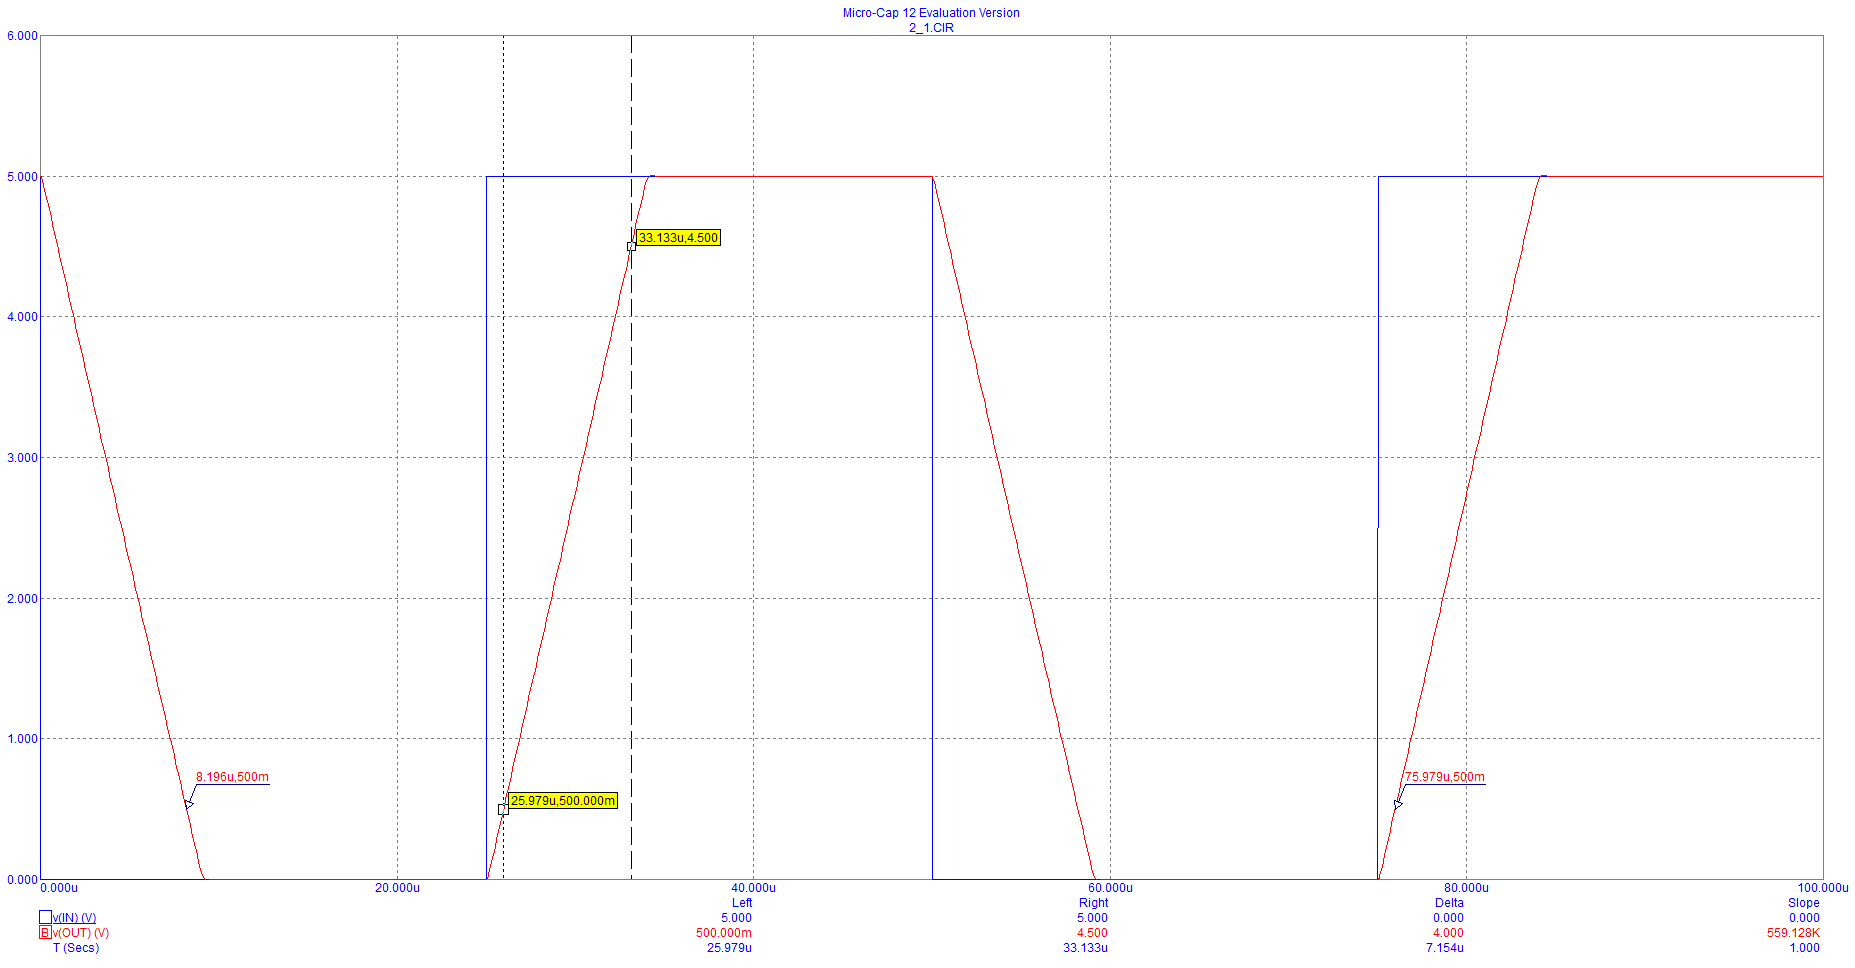
\includegraphics[width=\textwidth]{numerika/Buffer/2_SlewRate.png}
		\centering
		\caption{Buffer, simulace -- Reakce obvodu na náběžnou a sestupnou hranu.}
		\label{fig:b-s-slewrate}
	\end{figure}



\begin{figure}[h!]
	\centering
	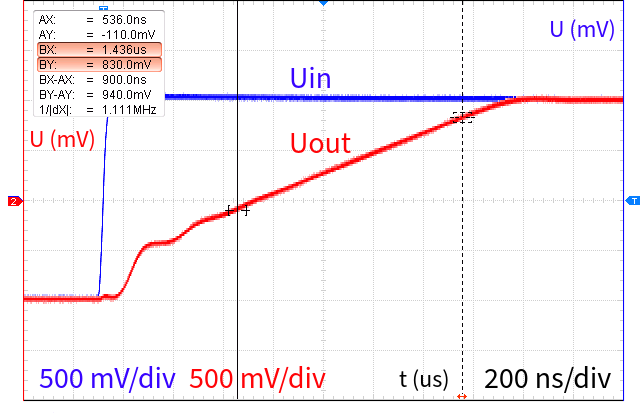
\includegraphics[width=\textwidth]{oscilo/output2.png}
	\centering
	\caption{Buffer, laboratoř -- Reakce obvodu na náběžnou hranu.}
	\label{fig:b-l-slewrate-nab}
\end{figure}

	\begin{figure}[h!]
	\centering
	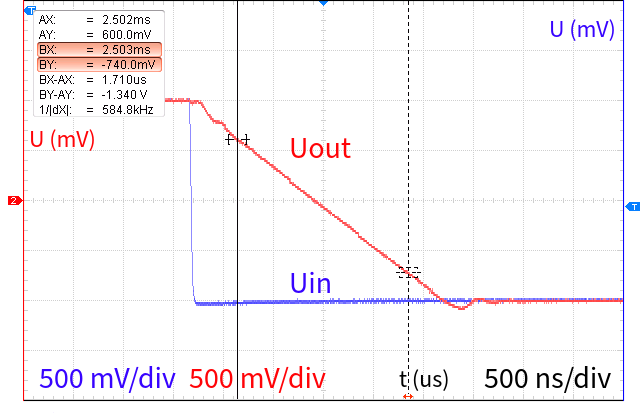
\includegraphics[width=\textwidth]{oscilo/output3.png}
	\centering
	\caption{Buffer, laboratoř -- Reakce obvodu na sestupnou hranu.}
	\label{fig:b-l-slewrate-ses}
\end{figure}

	Zapojení sledovače je ideální k měření mezní rychlosti přeběhu. Obr.~\ref{fig:b-s-slewrate} zobrazuje simulaci zkreslení obdélníkového signálu, výpočtem stanovíme mezní rychlost přeběhu, která je stejná pro náběžnou i sestupnou hranu:
$$ SR_{sim}=\frac{\Delta U}{\Delta t}=\frac{4,5-1,5}{33,133-25,979}\doteq \qty{0.419}{\volt\per\micro\second} $$


	Z Obr.~\ref{fig:b-l-slewrate-nab} a \ref{fig:b-l-slewrate-ses} stejným způsobem vypočteme hodnotu odpovídající měření v laboratoři, zvlášť pro náběžnou a sestupnou hranu:

$$ SR_{lab - rise}=\frac{\Delta U}{\Delta t}=\frac{0,830}{1,436}\doteq \qty{0.578}{\volt\per\micro\second} $$

$$ SR_{lab - fall}=\frac{\Delta U}{\Delta t}=\frac{0,740}{2503}\doteq \qty{0.296}{\volt\per\milli\second} $$

	

	\begin{figure}[h!]
		\centering
		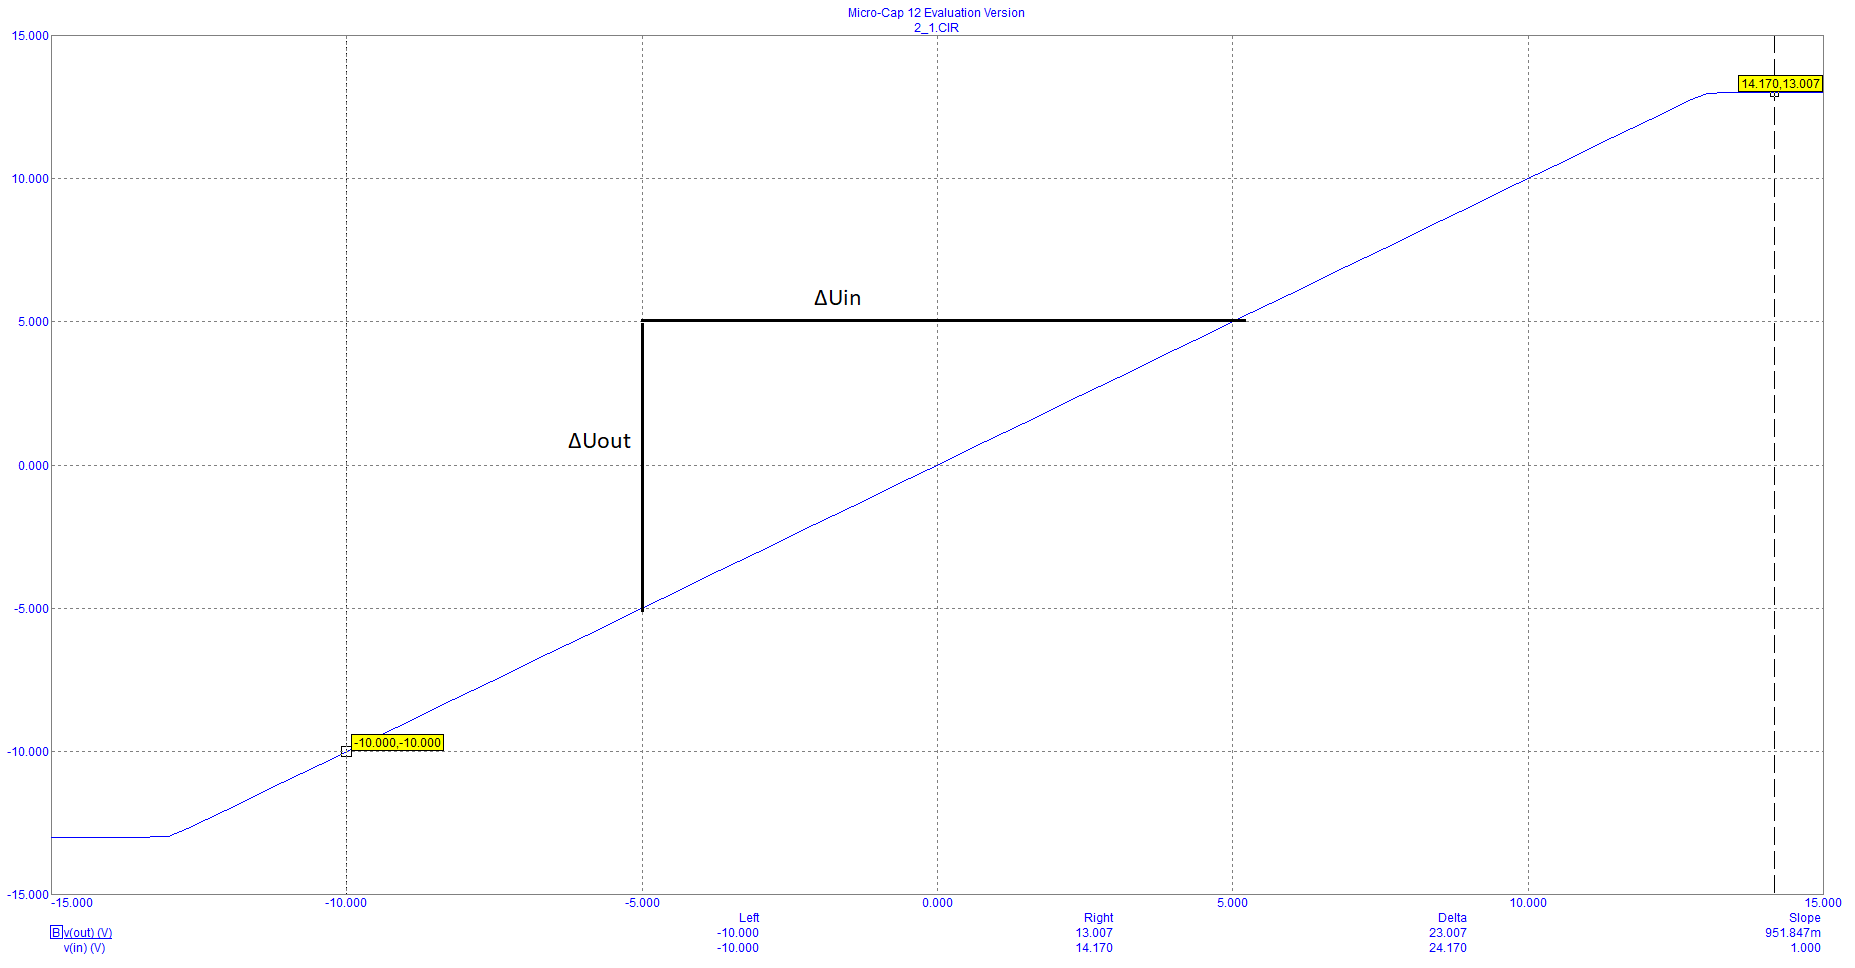
\includegraphics[width=0.9\textwidth]{numerika/Buffer/6_dc_zesileni_a_saturacni.png}
		\centering
		\caption{Buffer, simulace -- Převodní charakteristika.}
		\label{fig:b-s-prevodni}
	\end{figure}

	\begin{figure}[h!]
		\centering
		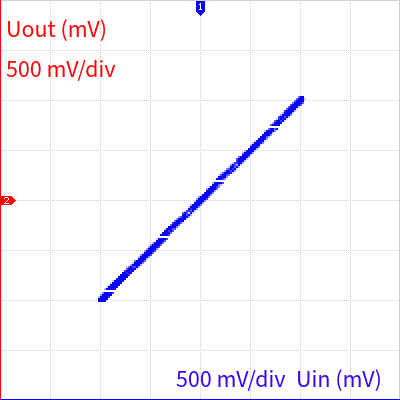
\includegraphics[width=0.5\textwidth]{oscilo/output4.png}
		\centering
		\caption{Buffer, laboratoř -- Převodní charakteristika.}
		\label{fig:b-l-prevodni}
	\end{figure}

Z převodních charakteristik na Obr.~\ref{fig:b-s-prevodni} a \ref{fig:b-l-prevodni} lze stanovit napěťové zesílení:

$$ A_{U - sim}=\frac{\Delta U_{in}}{\Delta U_{out}}=\frac{10}{10}=1$$
$$ A_{U - lab}=\frac{\Delta U_{in}}{\Delta U_{out}}=\frac{2}{2}=1$$





%\clearpage
\subsection{Neinvertující zesilovač}	
	\begin{figure}[h!]
		\centering
		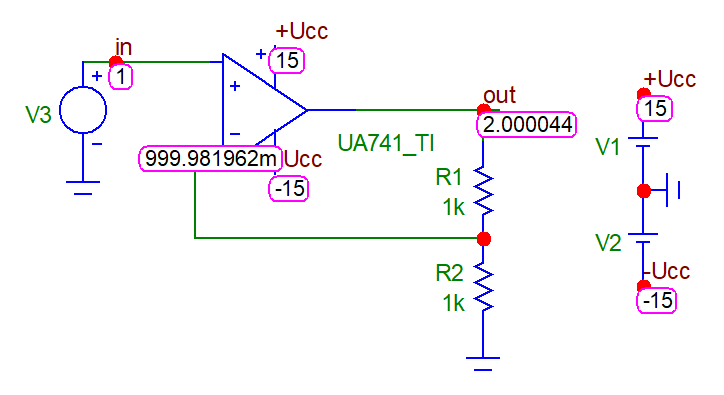
\includegraphics[width=\textwidth]{numerika/NonInverting/1_dc_prac_bod.png}
		\centering
		\caption{Neinvertující zes., simulace -- Pracovní bod obvodu.}
		\label{fig:ni-s-pracbod}
	\end{figure}
	
	\begin{figure}[h!]
		\centering
		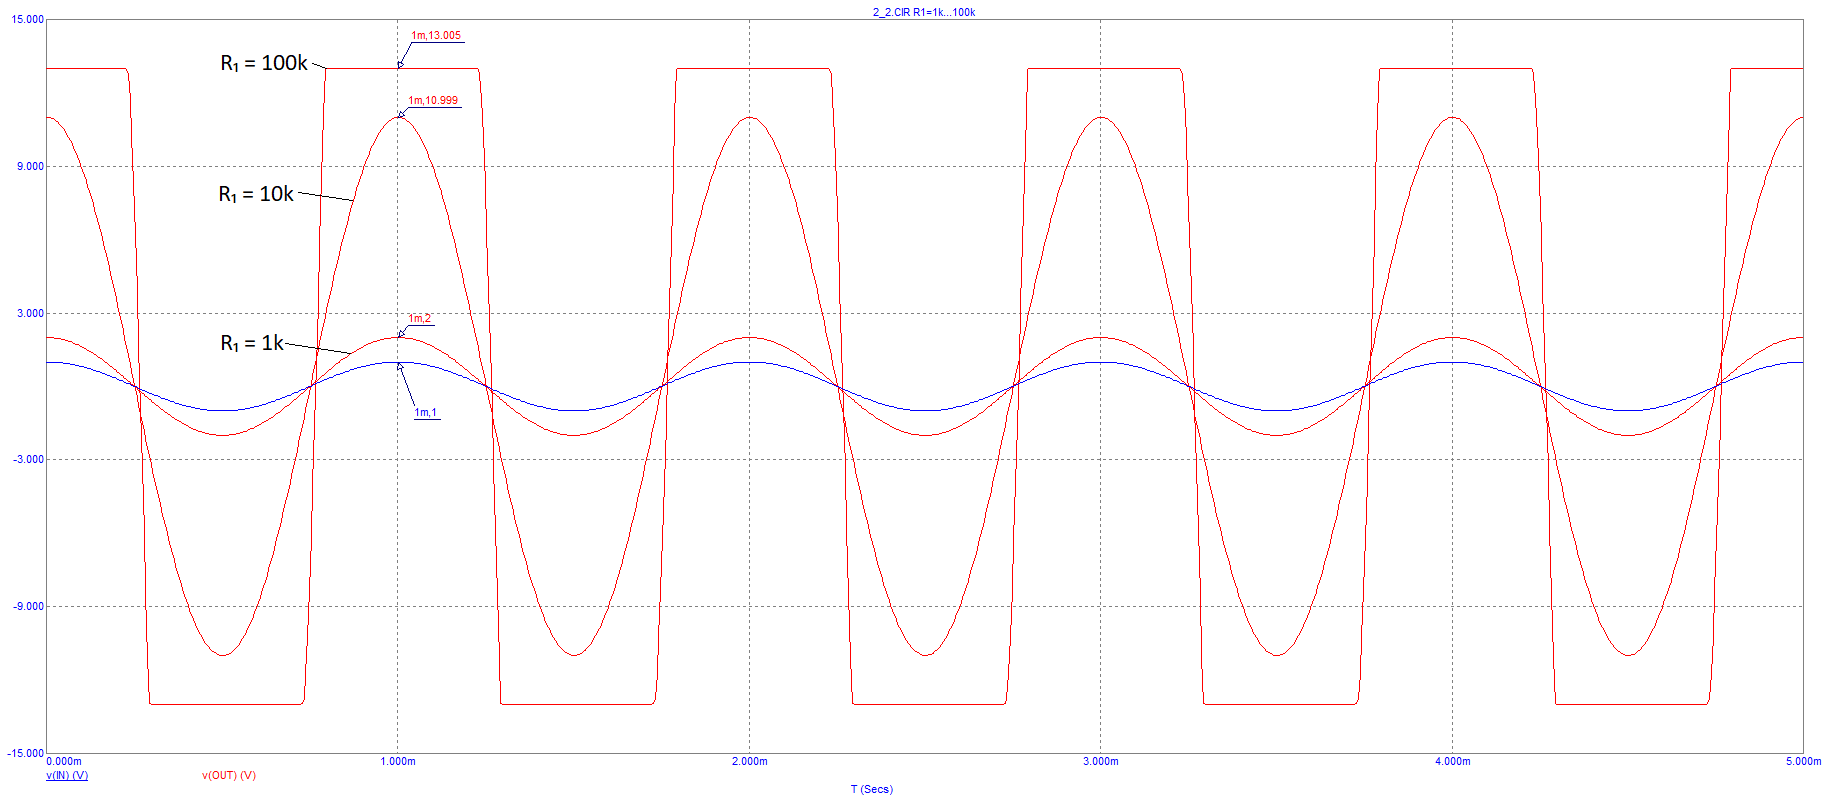
\includegraphics[width=\textwidth]{numerika/NonInverting/2_transient.png}
		\centering
		\caption{Neinvertující zes., simulace -- Přenos signálu o frekvenci \qty{100}{\kilo\hertz} pro různá zesílení, $ R_{1}= \{\SI{1}{\kilo\ohm};\SI{10}{\kilo\ohm};\SI{100}{\kilo\ohm}\} $.}
		\label{fig:ni-s-prenos}
	\end{figure}
	
	
	
\begin{figure}[h!]
	\centering
	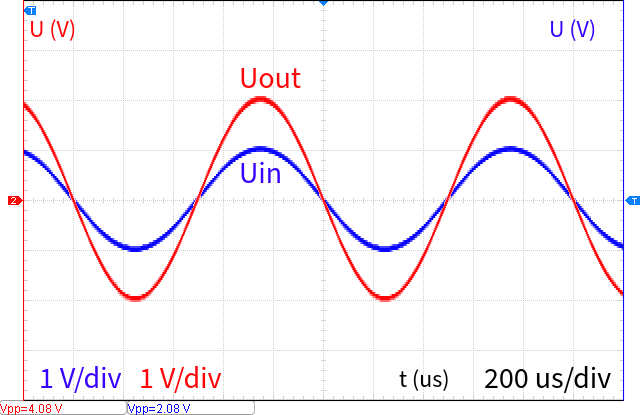
\includegraphics[width=\textwidth]{oscilo/output5.png}
	\centering
	\caption{Neinvertující zesilovač -- vstupní a výstupní signál v čase, $R_1=R_2=\SI{1}{\kilo\ohm}$}
	\label{fig:ni-l-prenos-1k}
\end{figure}

\begin{figure}[h!]
	\centering
	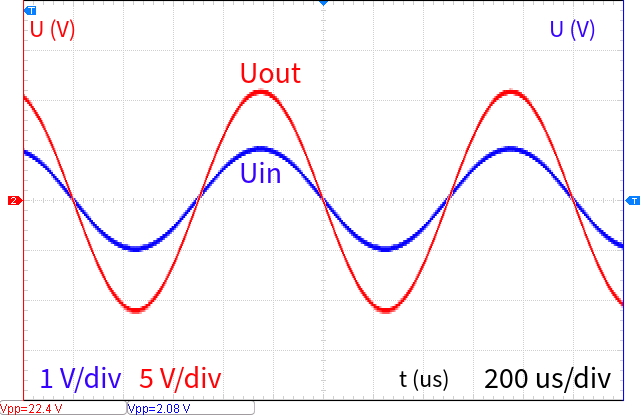
\includegraphics[width=\textwidth]{oscilo/output6.png}
	\centering
	\caption{Neinvertující zesilovač -- vstupní a výstupní signál v čase, $R_1=\SI{10}{\kilo\ohm}$, $R_2=\SI{1}{\kilo\ohm}$}
	\label{fig:ni-l-prenos-10k}
\end{figure}

\begin{figure}[h!]
	\centering
	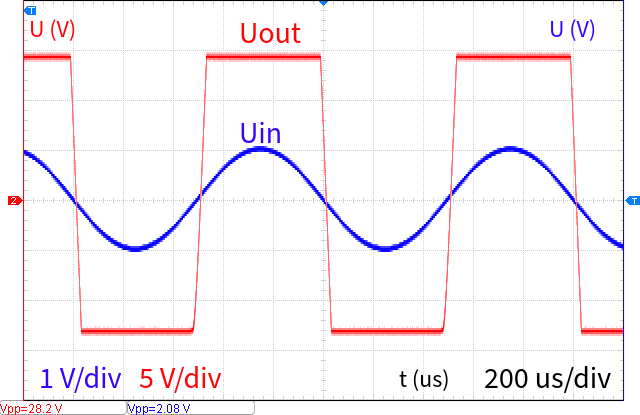
\includegraphics[width=\textwidth]{oscilo/output7.png}
	\centering
	\caption{Neinvertující zesilovač -- vstupní a výstupní signál v čase, $R_1=\SI{100}{\kilo\ohm}$, $R_2=\SI{1}{\kilo\ohm}$}
	\label{fig:ni-l-prenos-100k}
\end{figure}

Z časových průběhů pomocí podílu amplitud (resp. hodnot P-P) vypočteme napěťové zesílení pro zapojení s jednotlivými odpory, obecně lze říci, že $ A_U=\frac{u_2}{u_1} $. Obdobně lze zesílení získat ze sklonu křivek na Obr.~\ref{fig:ni-s-prenos}. Vypočtené hodnoty jsou uvedeny v Tab.~\ref{tab:hodnoty-zesileni-ni}. Pro případ, kdy $ R_1=\qty{100}{\kilo\ohm}$ nejsou některé výsledky uvedeny, protože zde působí silné zkreslení signálu vlivem dosažení saturačního napětí.



\begin{figure}[h!]
	\centering
	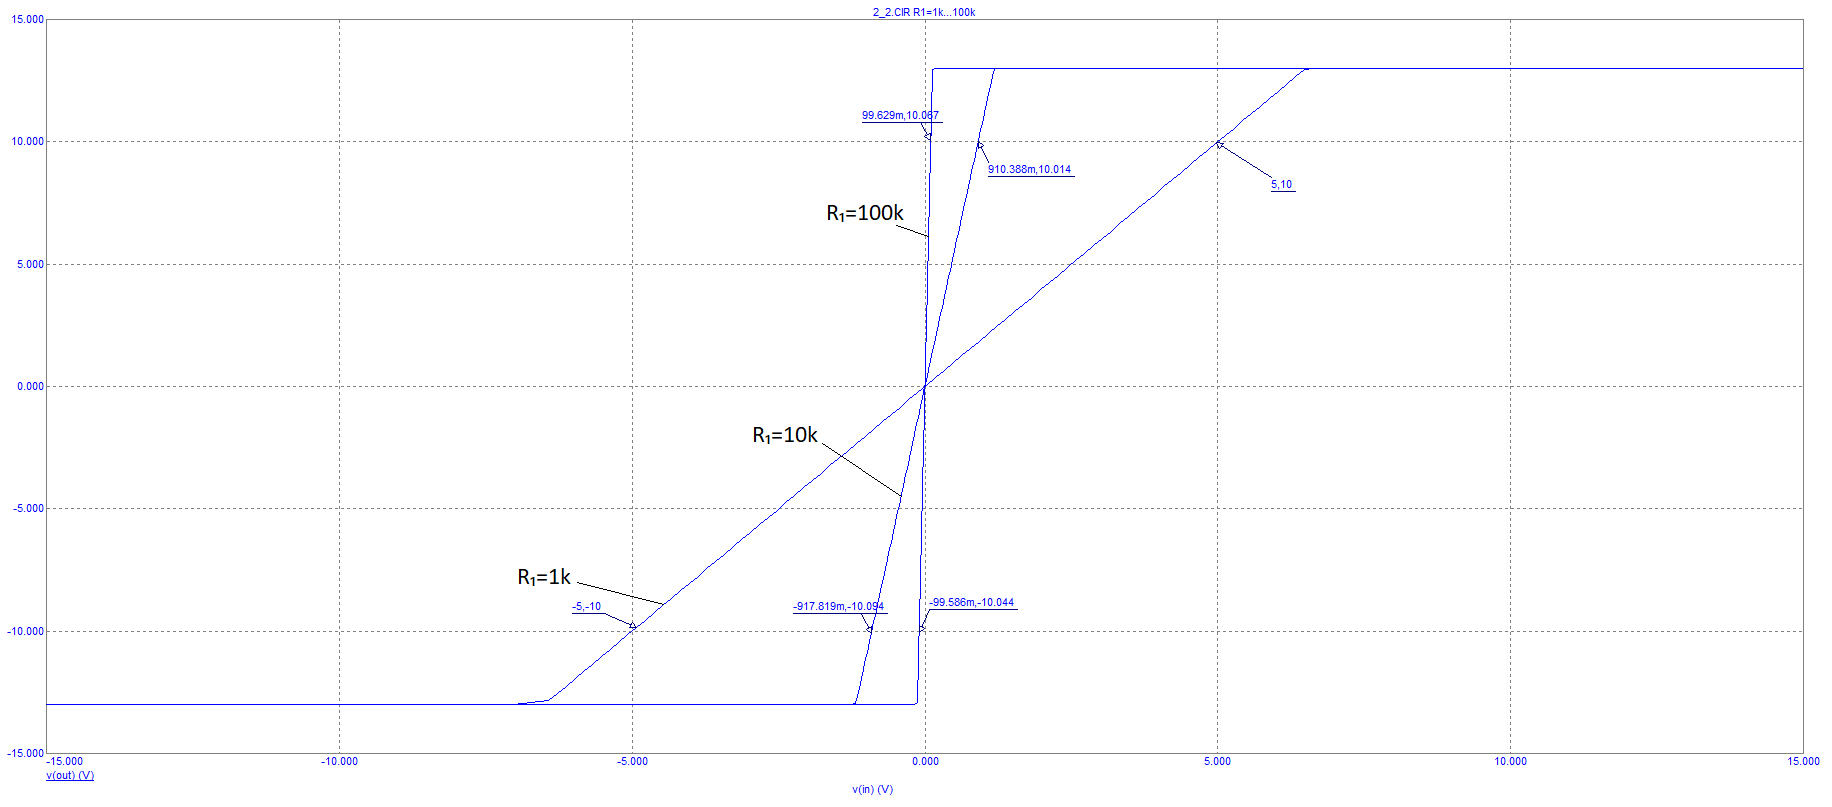
\includegraphics[width=\textwidth]{numerika/NonInverting/4_dc_zesileni.png}
	\centering
	\caption{Neinvertující zes., simulace -- Převodní charakteristika zapojení pro různé hodnoty $ R_1 $.}
	\label{fig:ni-s-prevodni}
\end{figure}

\begin{figure}
	\centering
\begin{minipage}{.45\textwidth}
	\centering
	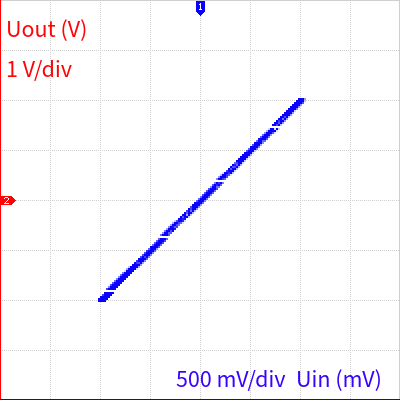
\includegraphics[width=\linewidth]{oscilo/output8.png}
	\captionof{figure}{Neinvertující zesilovač -- převodní charakteristika, $R_1=R_2=\SI{1}{\kilo\ohm}$}
	\label{fig:ni-l-prevodni-1k}
\end{minipage}%
\hspace{.09\textwidth}
\begin{minipage}{.45\textwidth}
	\centering
	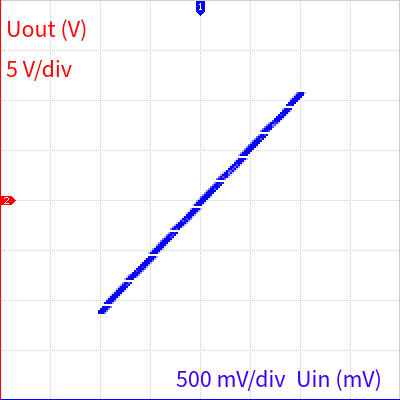
\includegraphics[width=\linewidth]{oscilo/output9.png}
	\captionof{figure}{Neinvertující zesilovač -- převodní charakteristika, $R_1=\SI{10}{\kilo\ohm}$, $R_2=\SI{1}{\kilo\ohm}$}
	\label{ni-l-prevodni-10k}
\end{minipage}
\end{figure}



\begin{figure}[h!]
	\centering
	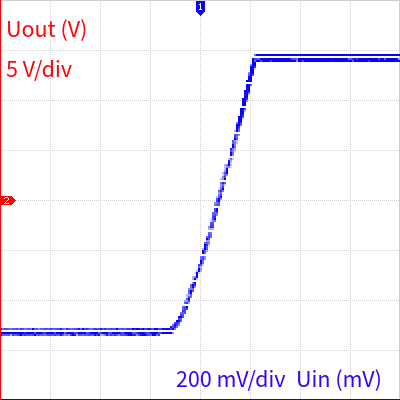
\includegraphics[width=0.5\textwidth]{oscilo/output10.png}
	\centering
	\caption{Neinvertující zesilovač -- převodní charakteristika, $R_1=\SI{100}{\kilo\ohm}$, $R_2=\SI{1}{\kilo\ohm}$}
	\label{fig:ni-l-prevodni-100k}
\end{figure}

\begin{table}[h!]
	\centering
	\def\arraystretch{1.4}
	\centering
	\begin{tabular}{|c|c|c|c|}	
		\hline
		$R_1 \; [\unit{\kilo\ohm}]$ & 1 & 10 & 100 \\ [0.1ex]
		\hline
		Simulace, časový průběh (Obr.~\ref{fig:ni-s-prenos})   &2  & 11 & -\\ [0.1ex]
		\hline 
		Měření, časový průběh (Obr.~\ref{fig:ni-l-prenos-1k} - \ref{fig:ni-l-prenos-100k}) & 1,96 & 10,77 &  -\\[0.1ex]
		\hline
		Simulace, převodní char. (Obr.~\ref{fig:ni-s-prevodni})   & 2  & 11 & 100,95\\ [0.1ex]
		\hline 
		Měření, převodní char. (Obr.~\ref{fig:ni-l-prevodni-1k} - \ref{fig:ni-l-prevodni-100k})   & 2  & $ \approx 11 $ & $ \approx90 $\\ [0.1ex]
		\hline 
	\end{tabular}
	\caption{Porovnání výsledků.}
	\label{tab:hodnoty-zesileni-ni}
\end{table}


	
\clearpage
\subsection{Invertující zesilovač}	
	\begin{figure}[h!]
		\centering
		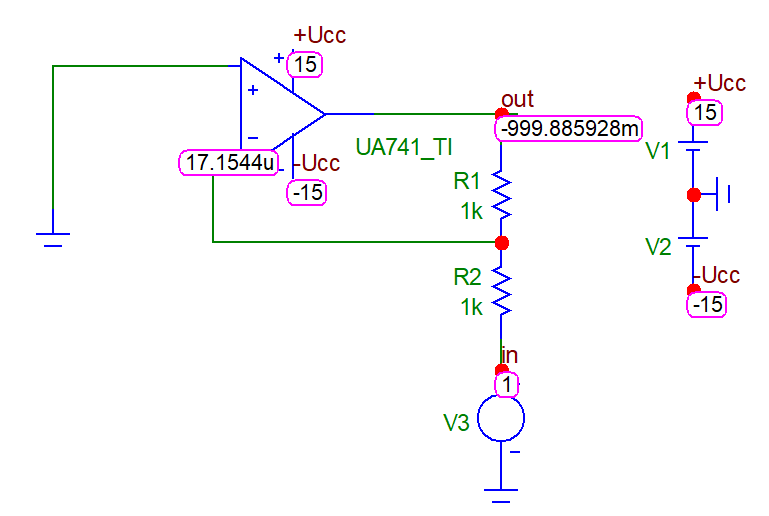
\includegraphics[width=\textwidth]{numerika/Inverting/1_dc_prac_bod.png}
		\centering
		\caption{Invertující zes., simulace -- Pracovní bod obvodu.}
		\label{fig:i-s-prac_bod}
	\end{figure}
	
	\begin{figure}[h!]
		\centering
		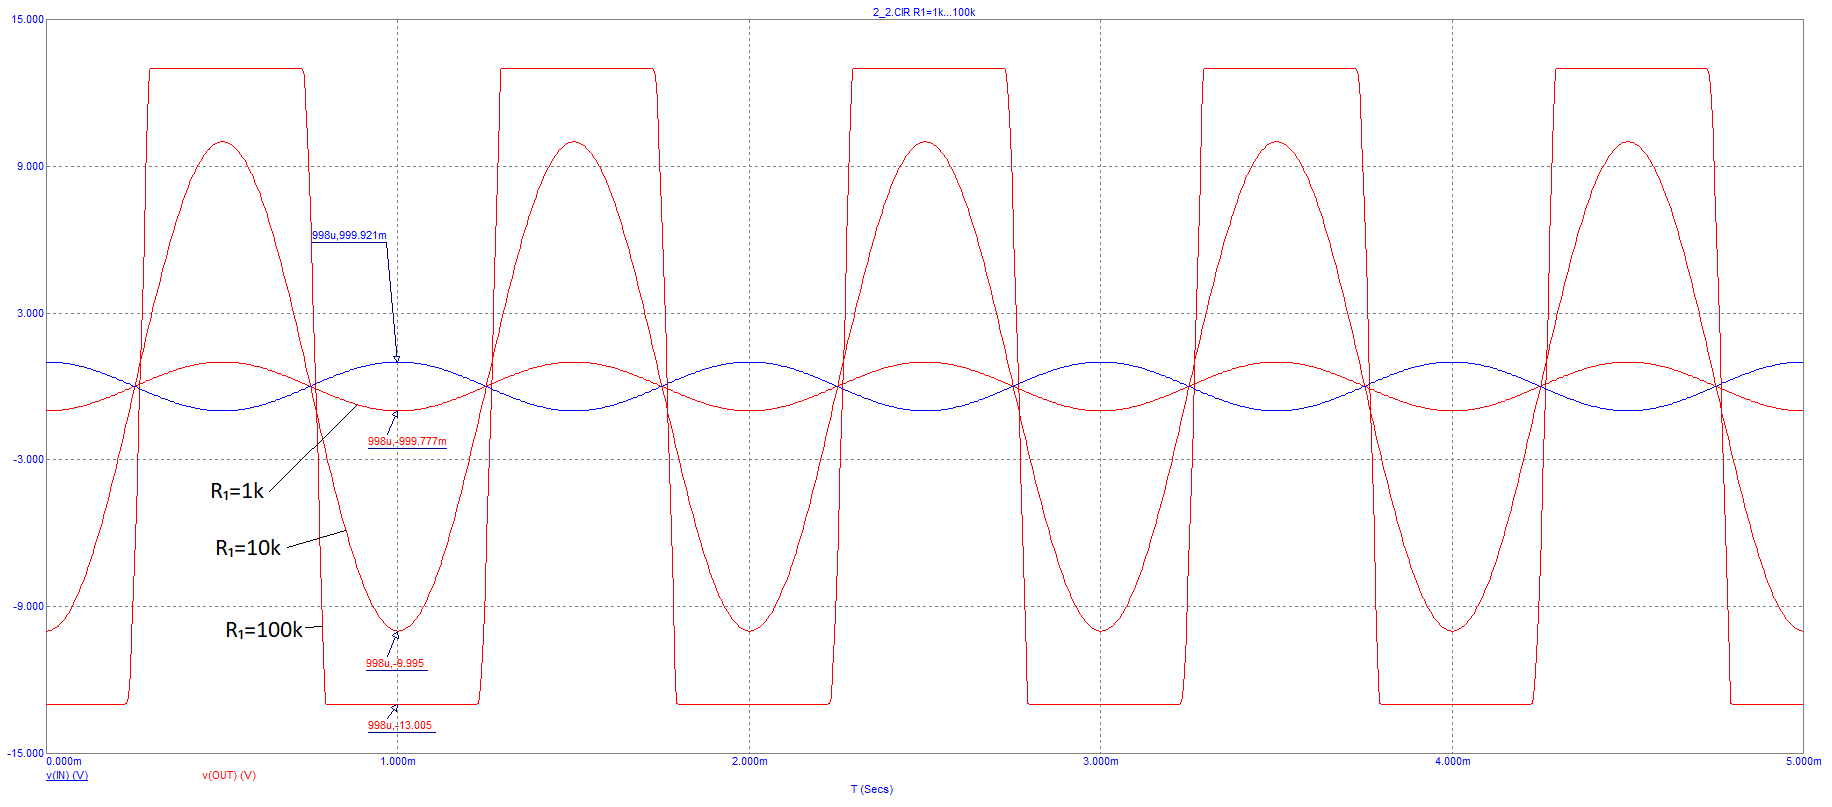
\includegraphics[width=\textwidth]{numerika/Inverting/2_transient.png}
		\centering
		\caption{Invertující zes., simulace -- Přenos signálu o frekvenci \qty{100}{\kilo\hertz} pro různá zesílení, $ R_{1}= \{\SI{1}{\kilo\ohm};\SI{10}{\kilo\ohm};\SI{100}{\kilo\ohm}\} $.}
		\label{fig:i-s-prenos}
	\end{figure}

\begin{figure}[h!]
	\centering
	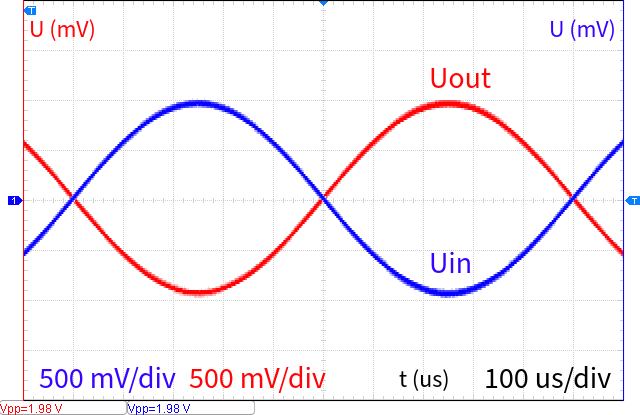
\includegraphics[width=\textwidth]{oscilo/output11.png}
	\centering
	\caption{Invertující zesilovač -- vstupní a	výstupní signál v čase, $R_1=R_2=\SI{1}{\kilo\ohm}$}
	\label{fig:i-l-prenos-1k}
\end{figure}

\begin{figure}[h!]
	\centering
	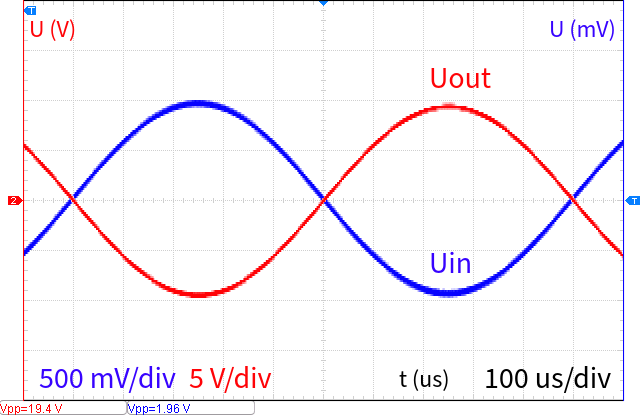
\includegraphics[width=\textwidth]{oscilo/output12.png}
	\centering
	\caption{Invertující zesilovač -- vstupní a	výstupní signál v čase, $R_1=\SI{10}{\kilo\ohm}$, $R_2=\SI{1}{\kilo\ohm}$}
	\label{fig:i-l-prenos-10k}
\end{figure}

\begin{figure}[h!]
	\centering
	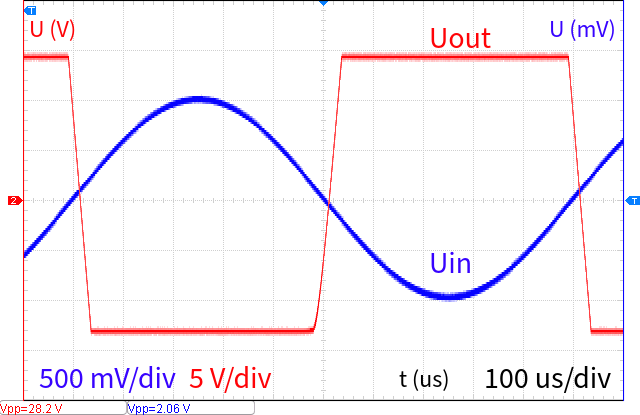
\includegraphics[width=\textwidth]{oscilo/output13.png}
	\centering
	\caption{Invertující zesilovač -- vstupní a	výstupní signál v čase, $R_1=\SI{100}{\kilo\ohm}$, $R_2=\SI{1}{\kilo\ohm}$}
	\label{fig:i-l-prenos-100k}
\end{figure}
	
	\begin{figure}[h!]
		\centering
		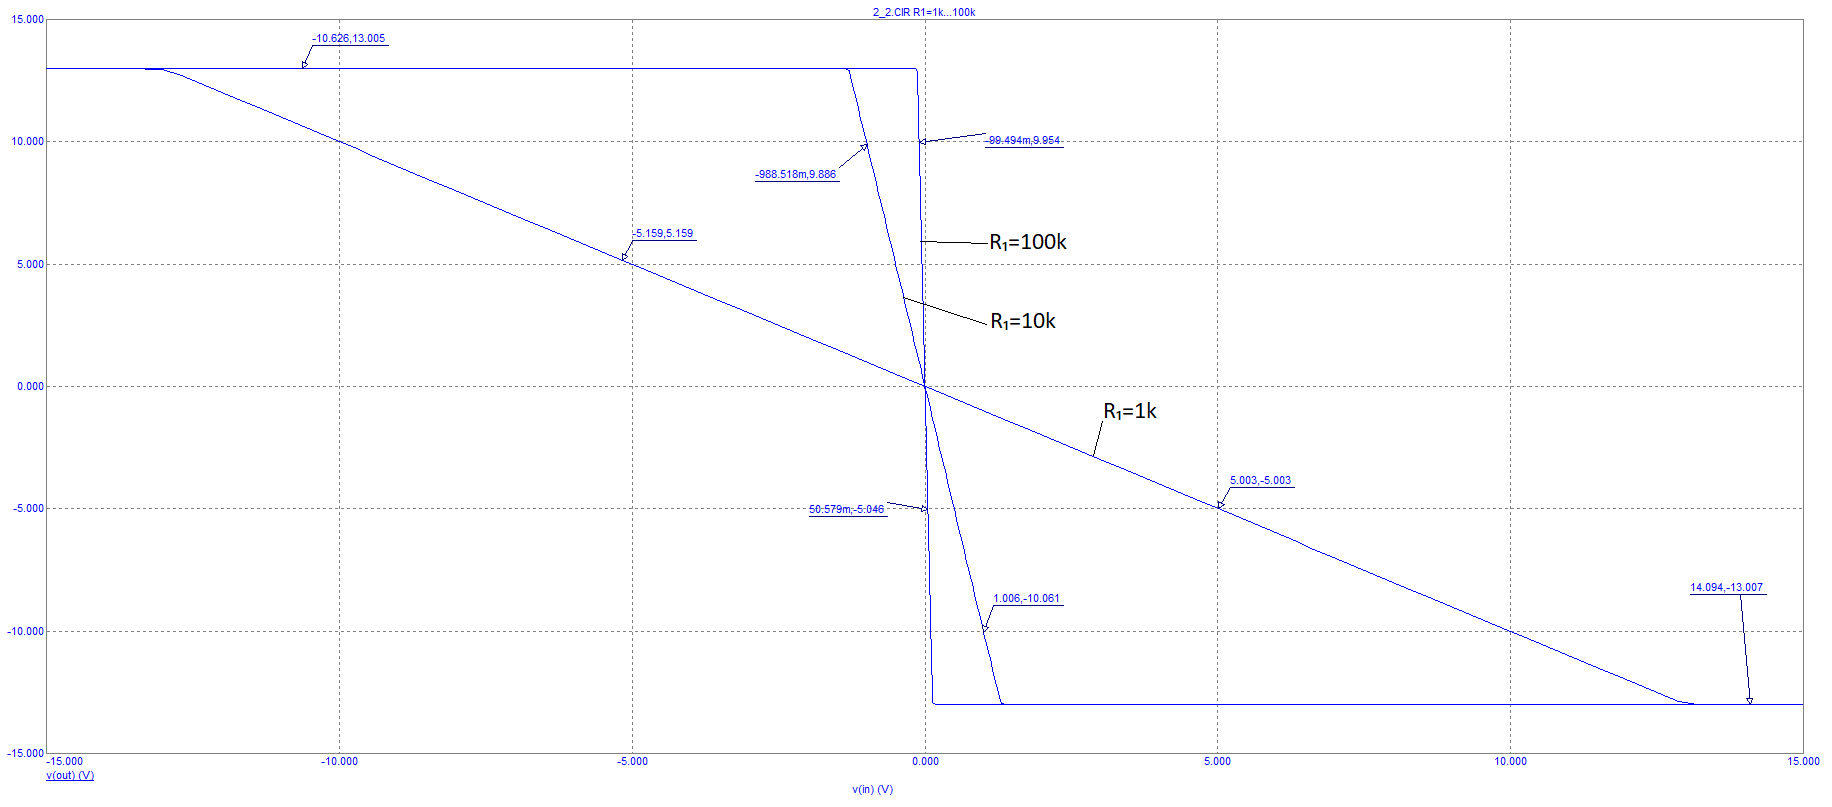
\includegraphics[width=\textwidth]{numerika/Inverting/3_dc_zesileni.png}
		\centering
		\caption{Invertující zes., simulace -- Převodní charakteristika.}
		\label{fig:i-s-prevodni}
	\end{figure}
	
		
		
		\begin{figure}
			\centering
			\begin{minipage}{.45\textwidth}
				\centering
				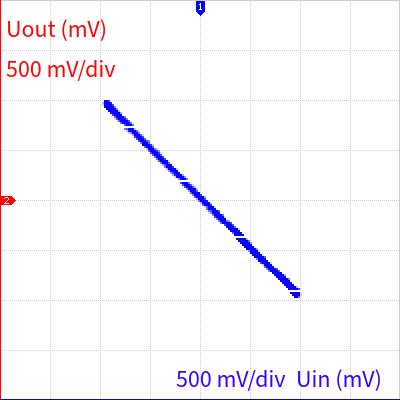
\includegraphics[width=\linewidth]{oscilo/output14.png}
				\captionof{figure}{Invertující zesilovač -- převodní charakteristika, $R_1=R_2=\SI{1}{\kilo\ohm}$}
				\label{fig:i-l-prevodni-1k}
			\end{minipage}%
			\hspace{.09\textwidth}
			\begin{minipage}{.45\textwidth}
				\centering
				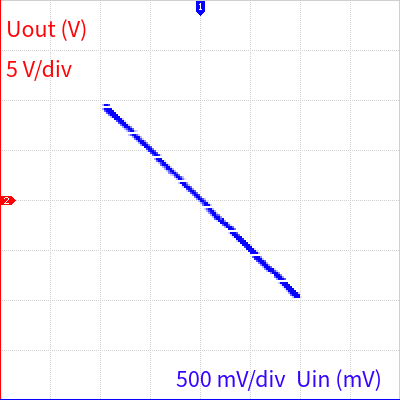
\includegraphics[width=\linewidth]{oscilo/output15.png}
				\captionof{figure}{Invertující zesilovač -- převodní charakteristika, $R_1=\SI{10}{\kilo\ohm}$, $R_2=\SI{1}{\kilo\ohm}$}
				\label{fig:i-l-prevodni-10k}
			\end{minipage}
		\end{figure}
		
		
	
	
	\begin{figure}[h!]
		\centering
		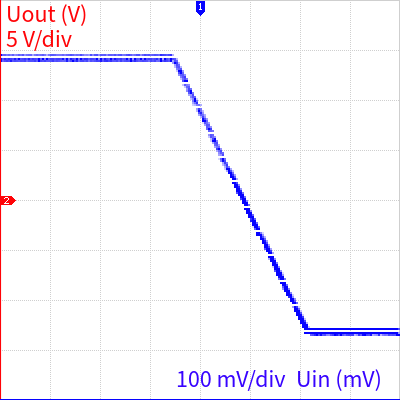
\includegraphics[width=0.5\textwidth]{oscilo/output16.png}
		\centering
		\caption{Invertující zesilovač -- převodní charakteristika, $R_1=\SI{100}{\kilo\ohm}$, $R_2=\SI{1}{\kilo\ohm}$}
		\label{fig:i-l-prevodni-100k}
	\end{figure}
	
	
	Obdobně jako pro zapojení neinvertujícho zesilovače vypočteme napěťové zesílení, postup je totožný. Získané hodnoty se nacházejí v Tab.~\ref{tab:hodnoty-zesileni-i}.
	
	\begin{table}[h!]
		\centering
		\def\arraystretch{1.4}
		\centering
		\begin{tabular}{|c|c|c|c|}	
			\hline
			$R_1 \; [\unit{\kilo\ohm}]$ & 1 & 10 & 100 \\ [0.1ex]
			\hline
			Simulace, časový průběh (Obr.~\ref{fig:i-s-prenos})   & -1  & -10 & -\\ [0.1ex]
			\hline 
			Měření, časový průběh (Obr.~\ref{fig:i-l-prenos-1k} - \ref{fig:i-l-prenos-100k}) & -1 & -9,9 &  -\\[0.1ex]
			\hline
			Simulace, převodní char. (Obr.~\ref{fig:i-s-prevodni})   & -1 & -10 & -99,95\\ [0.1ex]
			\hline 
			Měření, převodní char. (Obr.~\ref{fig:i-l-prevodni-1k} - \ref{fig:i-l-prevodni-100k})   & -1 & $ \approx -10 $ & $ \approx -100$\\ [0.1ex]
			\hline 
		\end{tabular}
		\caption{Porovnání výsledků.}
		\label{tab:hodnoty-zesileni-i}
	\end{table}
	
\clearpage	
\section{Kmitočtové charakteristiky}	
	
\begin{figure}[h!]
	\centering
	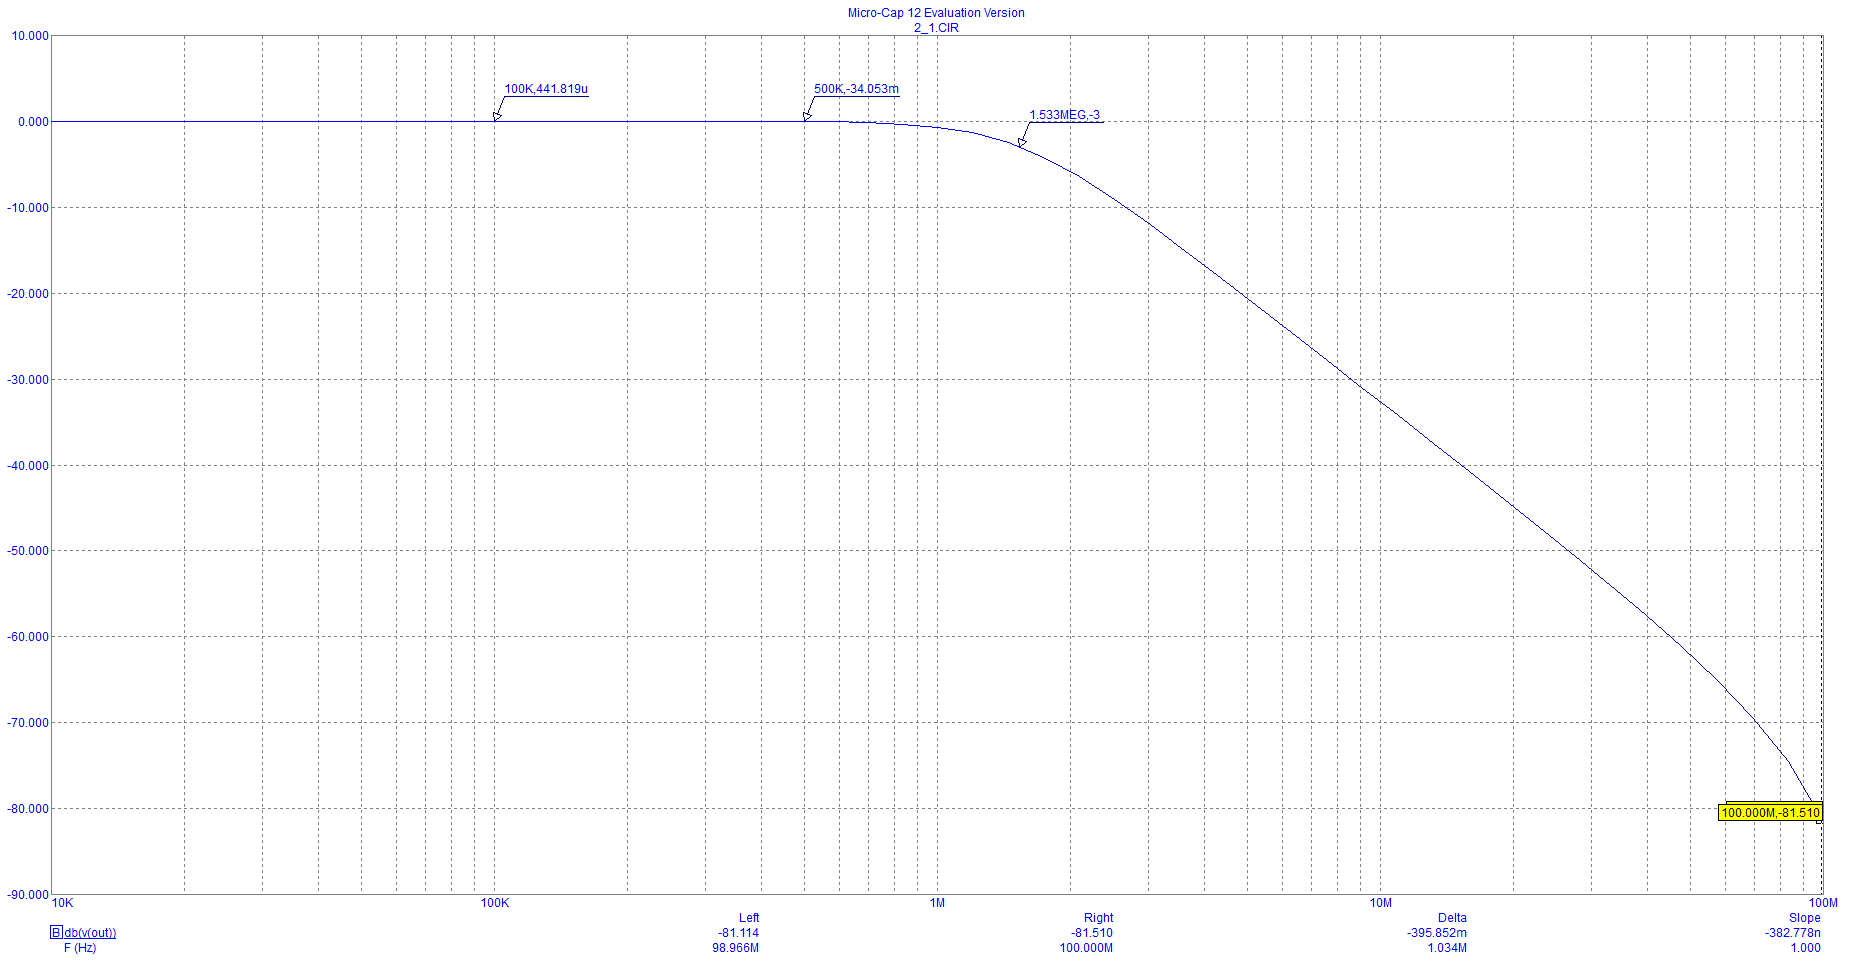
\includegraphics[width=\textwidth]{numerika/Buffer/5_kmitoctova_char.png}
	\centering
	\caption{Buffer, simulace -- Kmitočtová charakteristika.}
	\label{fig:b-s-kmitoctova}
\end{figure}


\begin{figure}[h!]
	\centering
	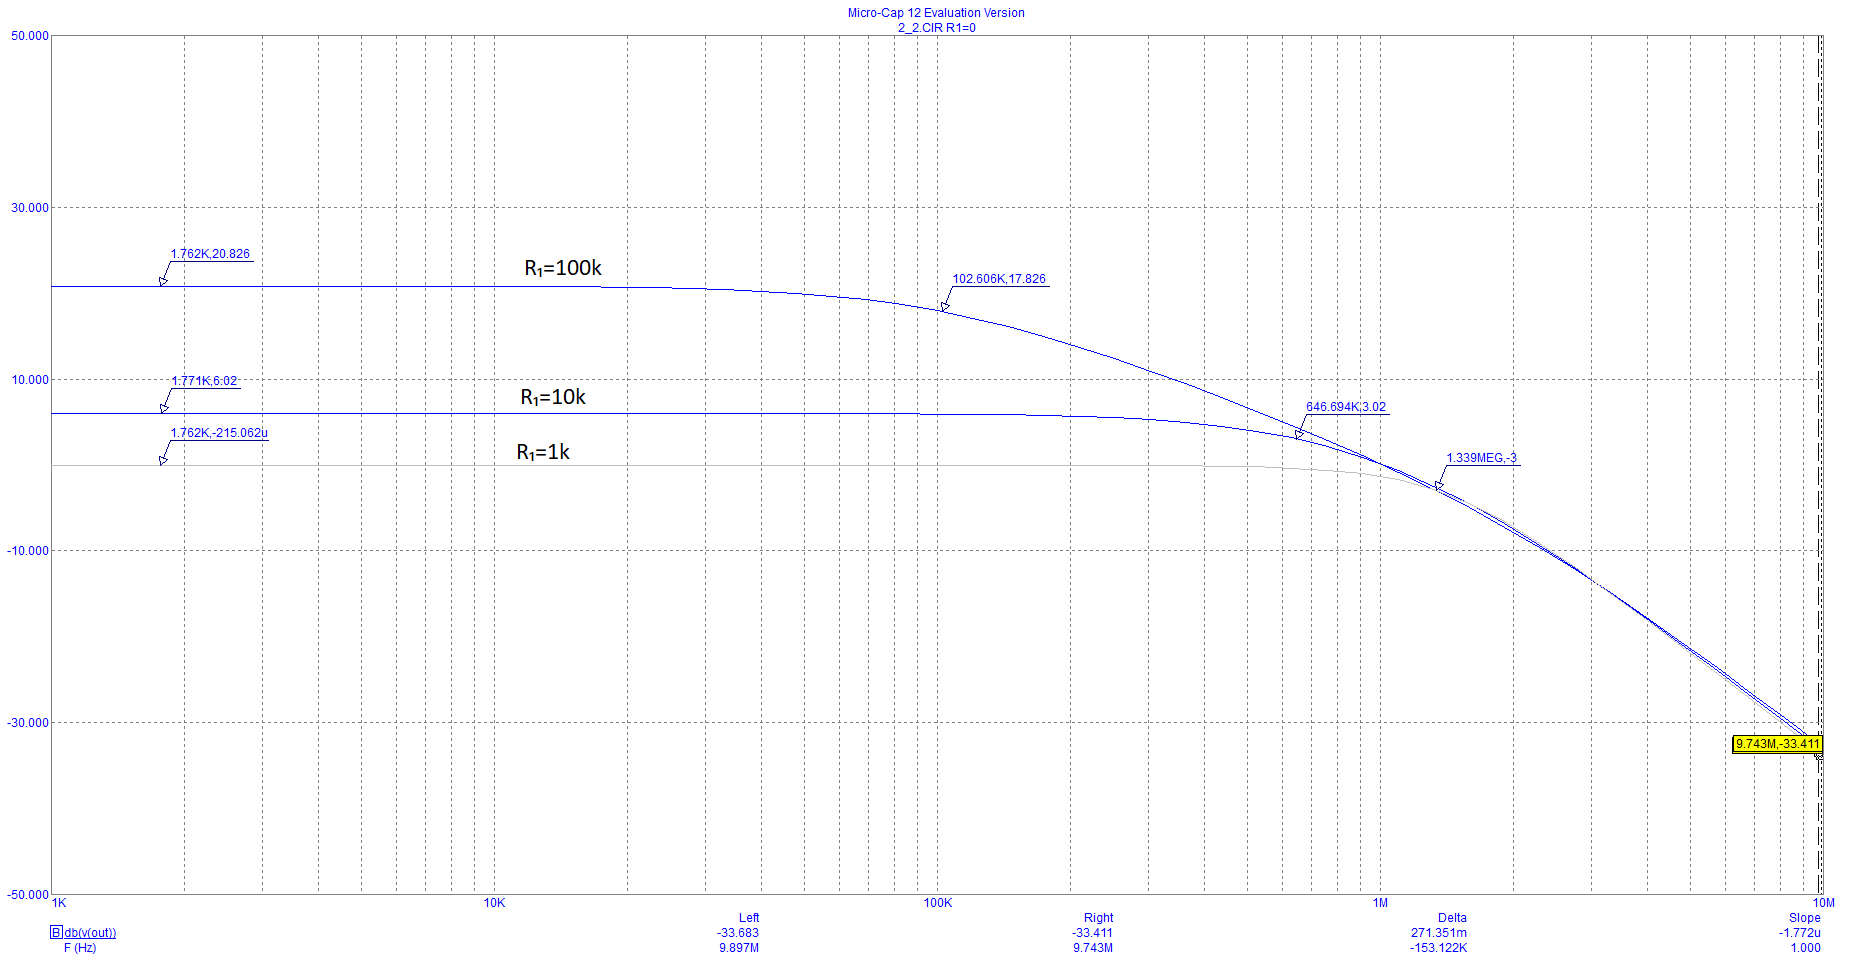
\includegraphics[width=\textwidth]{numerika/NonInverting/5_kmitoctova_char.png}
	\centering
	\caption{Neinvertující zes., simulace -- Kmitočtová charakteristika.}
	\label{fig:ni-s-kmitoctova}
\end{figure}
	
\begin{figure}[h!]
	\centering
	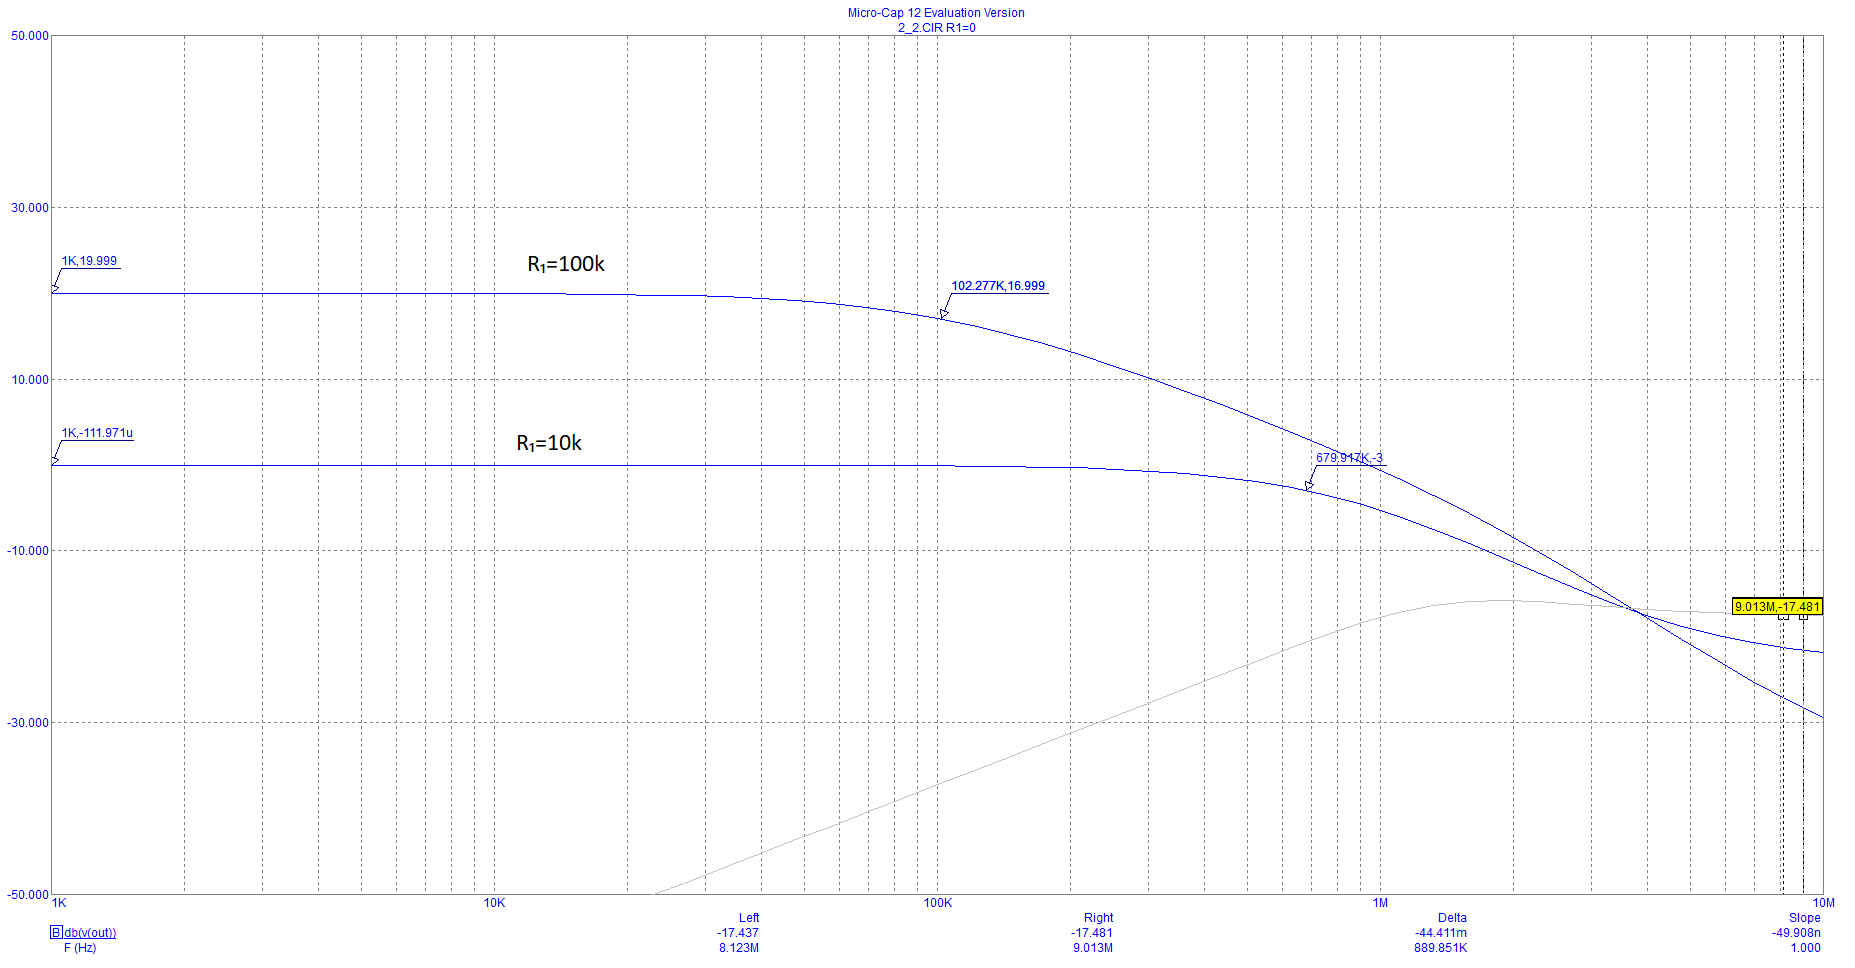
\includegraphics[width=\textwidth]{numerika/Inverting/4_kmitoctova_char.png}
	\centering
	\caption{Invertující zes., simulace -- Kmitočtová charakteristika.}
	\label{fig:i-s-kmitoctova}
\end{figure}

	\begin{figure*}[h!]
		\begin{tikzpicture}
			\centering
			\begin{axis}
				[
				xlabel={$f\ [\unit{\kilo\hertz}]$},
				ylabel={$A_U\ [\unit{\deci\bel}]$},
				width=1\textwidth,
				height = 0.5\textwidth,
%				legend pos=south east,
				legend style={at={(0.015,0.025)},anchor=south west},
				xmode=log,
				xmin=1,
				xmax=1e4
				]
				% 4.7 muF
				\addplot[mark=x, blue, smooth, mark size=3pt] table [skip first n=2, x=f1, y=A1, col sep=comma] {data/data.csv};
				\addlegendentry{Neinvertující zes., $R_1=\SI{10}{\kilo\ohm}$, $R_2=\SI{1}{\kilo\ohm}$}
				% 10 muF
				\addplot[mark=x, red, smooth, mark size=3pt] table [skip first n=2, x=f2, y=A2, col sep=comma] {data/data.csv};
				\addlegendentry{Invertující zes.								, $R_1=\SI{10}{\kilo\ohm}$, $R_2=\SI{1}{\kilo\ohm}$}
				% 100 nF
				\addplot[mark=x, green, smooth, mark size=3pt] table [skip first n=2, x=f3, y=A3, col sep=comma] {data/data.csv};
				\addlegendentry{Buffer}
				
				% -3dB
				\addplot [
				domain=0.1:1e7, 
				samples=2, 
				color=gray,
				dashed,
				no marks
				]
				{-3};		
				
				% Proměnné pro popisky a vynášecí čáry
				\def\firstx{330}
				\def\secondx{5.5}
				\def\thirdx{235}
				\def\fourthx{4.5e5}
				\def\topy{-2.1}
				\def\bottomy{-17}
				\def\labeltop{-15.9}
				
				\node[] (A) at (axis cs: \firstx,\bottomy) {};
				\node[] (Alabel) at (axis cs: \firstx,\labeltop) {};
				\node[] (AA) at (axis cs: \firstx,\topy) {};
%				\node[] (B) at (axis cs: \secondx,\bottomy) {};
%				\node[] (Blabel) at (axis cs: \secondx,\labeltop) {};
%				\node[] (BB) at (axis cs: \secondx,\topy) {};
%				\node[] (C) at (axis cs: \thirdx,\bottomy) {};
%				\node[] (Clabel) at (axis cs: \thirdx,\labeltop) {};
%				\node[] (CC) at (axis cs: \thirdx,\topy) {};
%				\node[] (D) at (axis cs: \fourthx,\bottomy) {};
%				\node[] (Dlabel) at (axis cs: \fourthx,\labeltop) {};
%				\node[] (DD) at (axis cs: \fourthx,\topy) {};
				\node[] (Elabel) at (axis cs: 1000,-3) {};

			\end{axis}    
		
		\node[anchor=north] (label) at (Alabel) {\SI{330}{\kilo\hertz}};
%		\node[anchor=north west] (label) at (Blabel) {\SI{5.5}{\hertz}};
%		\node[anchor=north west] (label) at (Clabel) {\SI{235}{\hertz}};
%		\node[anchor=north east] (label) at (Dlabel) {\SI{4.5e5}{\hertz}};
		\node[anchor=south west] (label) at (Elabel) {\SI{-3}{\deci\bel}};
		\draw (A) -- (AA);
%		\draw (B) -- (BB);
%		\draw (C) -- (CC);
%		\draw (D) -- (DD);
		
		\end{tikzpicture}
		\caption{Kmitočtová charakteristika OZ pro aplikace s různým zesílením.}
		\label{fig:graf_fajny}
	\end{figure*}


\clearpage


\section{Závěr}
\subsubsection{Buffer}
Pro zapojení sledovače jsme měřili napěťové zesílení, díky záporné zpětné vazbě musí být na výstupu stejná hodnota napětí jako na vstupu, zesílení je tedy $ A_U=1 $, což jsme ověřili jak počítačvovou simulací, tak i měřením.

Toto zesílení je ale frekvenčně závislé. Obr.~\ref{fig:b-s-prenos1} a \ref{fig:b-s-prenos2} zobrazují simulaci přenosu signálu o různých frekvencích, pro frekvenci \qty{500}{\kilo\hertz} je vidět, že signál je již značně utlumený, což odporuje kmitočtové charakteristice vytvořené simulací (Obr.~\ref{fig:b-s-kmitoctova}), ale je to v souladu s námi změřenou charakteristikou. Modul simulace frekvenční charakteristiky tedy nejspíše nezapočítává některý důležitý parametr. Rozdíl v simulované a měřené šířce pásma je nezanedbatelný a z mého pohledu je tento modul simulace nepoužitelný, jelikož je v rozporu jak s měřeními, tak i s dalšími moduly simulace. Vlastním měřením jsme tedy stanovili tranzitní kmitočet $ f_t=\qty{330}{\kilo\hertz} $. Výrobce udává podstatně vyšší hodnotu, zde může mít vliv také mezní rychlost přeběhu, která pro vyšší frekvence způsobuje nelineární zkreslení, pokud je použita příliš velká amplituda.

Tento parametr jsme určovali z reakce obvodu na obdélníkový impuls, v simulaci nám vyšla hodnota $ SR_{sim}\doteq \qty{0.419}{\volt\per\micro\second} $, ta je zde stejná pro náběžnou i sestupnou hranu. V laboratoři jsme pak naměřili hodnoty $ SR_{lab - rise}\doteq \qty{0.578}{\volt\per\micro\second} $ pro náběžnou hranu a $ SR_{lab - fall}\doteq \qty{0.296}{\volt\per\milli\second} $ pro sestupnou -- ta vyšla o několik řádů nižší.

\subsubsection{Neinvertující zesilovač}
Zde jsme měnili poměr hodnot zpětnovazebních odporů, čímž jsme nastavovali zesílení obvodu. Tab.~\ref{tab:hodnoty-zesileni-ni} porovnává dosažené výsledky. Simulace i měření si vzájemně odpovídají, ověřili jsme také použití teoretického vztahu pro výpočet $ A_U = 1+\frac{R_1}{R_2} $. Z převodní charakteristiky je také možné odečíst saturační napětí, které odpovídá $ \approx 13-14 $\ V, tedy o 1 -- 2\ V méně, než je napětí napětí napájecí.%
%
\subsubsection{Invertující zesilovač}
Pro toto zapojení je situace obdobná, z časových průběhů je zřejmé, že zesílení opět závisí na poměru zpětnovazebních odporů a výstupí signál je navíc invertovaný. Zjištěné hodnoty $ A_U $ se nacházejí v Tab.~\ref{tab:hodnoty-zesileni-i}. I zde jsme ověřili použitelnost teoretického vztahu, tentokrát vztahu $ A_U=-\frac{R_1}{R_2} $.

\begin{table}[h!]
	\centering
	\def\arraystretch{1.4}
	\centering
	\begin{tabular}{|c|c|c|c|}	
		\hline
		& $f_t \; [\unit{kHz}]$ & $SR_{rise} \; [\unit{\volt\per\micro\second}]$ & $SR_{fall} \; [\unit{\volt\per\micro\second}]$  \\ [0.1ex]
		\hline
		Simulace  & \num{1533} & 0,419 & 0,419 \\[0.1ex]
		\hline
		Měření    & 133 & 0,578 & \num{0,296e-3} \\[0.1ex]
		\hline
	\end{tabular}
	\caption{Srovnání ostatních parametrů.}
	\label{tab:porovnani-ostatni}
\end{table}

\end{document} 
